\documentclass[twoside,a4paper]{article}
\usepackage{geometry}
\geometry{margin=1.5cm, vmargin={0pt,1cm}}
\setlength{\topmargin}{-1cm}
\setlength{\paperheight}{29.7cm}
\setlength{\textheight}{25.3cm}

% useful packages.
\usepackage{amsfonts}
\usepackage{amsmath}
\usepackage{amssymb}
\usepackage{amsthm}
\usepackage{enumerate}
\usepackage{graphicx}
\usepackage{multicol}
\usepackage{fancyhdr}
\usepackage{layout}
\usepackage{tabularx}
\usepackage{xeCJK}

% some common command
\newcommand{\dif}{\mathrm{d}}
\newcommand{\avg}[1]{\left\langle #1 \right\rangle}
\newcommand{\difFrac}[2]{\frac{\dif #1}{\dif #2}}
\newcommand{\pdfFrac}[2]{\frac{\partial #1}{\partial #2}}
\newcommand{\OFL}{\mathrm{OFL}}
\newcommand{\UFL}{\mathrm{UFL}}
\newcommand{\fl}{\mathrm{fl}}
\newcommand{\op}{\odot}
\newcommand{\Eabs}{E_{\mathrm{abs}}}
\newcommand{\Erel}{E_{\mathrm{rel}}}

\begin{document}

\pagestyle{fancy}
\fancyhead{}
\lhead{俞璐 (3180104284)}
\chead{Project2-数学文档}
\rhead{2021/06/5}

\section*{I. 问题介绍}
\hspace{0.8em}
多重网格方法往往与求解微分方程相关,首先我们先假设之后的讨论都围绕下列的泊松方程展开
$$
    \begin{cases}
        -\Delta u(x)=f(x)\quad & x\in \Omega:=(0,1);  \\
        u(x)=g(x)\quad         & x\in \partial \Omega
    \end{cases}
$$
通过对该方程进行离散,我们将问题转化为求解一个线性系统
$$
    A\mathbf{u}=\mathbf{f}
$$
假设这个线性系统的精确解为$\tilde{\mathbf{u}}$,逼近解为$\mathbf{u}$,则我们可以定义误差为$\mathbf{e}=\mathbf{u}-\tilde{\mathbf{u}}$,残差为$\mathbf{r}=\mathbf{f}-A\tilde{\mathbf{u}}$,而此时问题可转化为求解
$$
    A\mathbf{e}=\mathbf{r}
$$
而原来的非齐次问题来说,通过这样的转化之后,变成了一个齐次问题。而多重网格方法能很好的求解这个问题。

\section*{II. 传统的迭代求解方法}
\hspace{0.8em}
很多传统的迭代方法本质上使用的是不动点迭代的方法,简要来说,对于求解$A\mathbf{u}=\mathbf{f}$,假设迭代格式为
$$\mathbf{u}^{(l+1)}=T\mathbf{u}^{(l)}+\mathbf{c}$$
则所对应的误差满足
$$\mathbf{e}^{(l)}=T^le^{(0)}$$
所以当$\rho(T)<1$时可以知道误差能够逼近0.
带权重的Jacobi就是非常经典的利用不动点迭代求解的方法,具体的迭代格式如下
\begin{align*}
    T                  & =-D^{-1}(L+U)                                  \\
    \mathbf{c}         & =D^{-1}\mathbf{f}                              \\
    \mathbf{u}^*       & =T\mathbf{u}^{(l)}+\mathbf{c}                  \\
    \mathbf{u}^{(l+1)} & =(1-\omega)\mathbf{u}^{(l)}+\omega\mathbf{u}^*
\end{align*}
其中$D,L,U$分别为$A$的对角线部分,下三角部分,上三角部分,而$\omega$则是权重,作为预先设置量提供.
进一步的我们可以有
$$
    T_\omega=(1-\omega)I-\omega D^{-1}(L+U)=I-\frac{\omega h^2}{2}A
$$
假如此时求解的$A$是上一部分我们说的泊松方程的线性系统的系数矩阵,那么由前一章的知识我们可以知道$A$的特征值和对应的特征向量$\lambda_k(A)$和$\omega_k$有
\begin{align*}
    \lambda_k(A) & =\frac{4}{h^2}\sin^2\frac{kh\pi}{2} \\
    \omega_{k,j} & =sin(x_jk\pi)
\end{align*}
从而我们可以知道$T_w$的特征值为$\lambda_k(T_\omega)=1-2\omega\sin^2\frac{k\pi}{2n}$,且对应的特征向量为$\omega_k$
显然这些特征向量是线性无关的,所以我们可以假设
$$
    \mathbf{e}^{(0)}=\sum_k c_k\omega_k
$$
则此时有
$$
    \mathbf{e}^{(l)}=\sum_k c_k\lambda_k^l(T_\omega)\omega_k
$$
其中当我们的网格逐渐加密的时候$\lambda_1=1-2\omega\sin^2\frac{\pi}{2n}\rightarrow 1$,所以此时初始误差中的低频部分很难被消除,而高频部分则很容易被消除.

\newpage
\section*{III. 多重网格方法}
\hspace{0.8em}
从第二部分我们可以看出带权重的Jacobi迭代很难消除误差中的低频部分,而多重网格能很好的消除低频部分.
\subsection*{III-a Restriction 和 Prolongation算子}
\hspace{0.8em}
因为之前的迭代方法能很好的处理高频部分,但是处理不了低频的部分,所以一个指导的想法就是将现在的低频部分转化为高频的部分,而这个可以通过
Restriction算子和Prolongation算子实现,简单来说这两个算子分别是将网格进行加粗和加密的操作,通过网格的加粗就可以将低频转化为高频,并通过Jacobi迭代将其消除,再通过加密操作将其恢复.

其中Restriction算子是$I^{2h}_h:\mathbb{R}^{n-1}\rightarrow\mathbb{R}^{\frac{n}{2}-1}$,具体的$I_{h}^{2h}$可以直接将$v_h$中的对应部分保留从而映射到$v^{2h}$,也可以是full-weighting算子$v_j^{2h}=\frac{1}{4}(v_{2j-1}^h+2v_{2j}^h+v_{2j+1}^h)$.

而Prolongation算子是$I^{h}_{2h}:\mathbb{R}^{\frac{n}{2}-1}\rightarrow\mathbb{R}^{n-1}$,其中$I_{2h}^{h}$可以使用线性插值也可以使用二次插值.

\subsection*{III-b V-cycle 和 FMG}
\hspace{0.9em}
具体两种算法的计算过程可见老师讲义.

\section*{IV. 理论分析}
\subsection*{IV-a 谱的角度}
\hspace{0.9em}
设$\mathbf{w}^h_k\left(k\in[1,\frac{n}{2})\right)$和$\mathbf{w}^h_{k'}(k'=n-k)$成为互补模式,$TG$算子为只有两层的V-cycle算子,$v_1,v_2$分别是V-cycle的参数(预先提供)以及$s_k:=\sin^2\frac{k\pi}{2n},c_k:=\cos^2\frac{k\pi}{2n}$,则通过一系列的推导我们有
\begin{align*}
    TG\mathbf{w}_k=\lambda_k^{v_1+v_2}s_k\mathbf{w}_k+\lambda_k^{v_1}\lambda_{k'}^{v_2}s_k\mathbf{w}_{k'} \\
    TG\mathbf{w}_{k'}=\lambda_{k'}^{v_1}\lambda_k^{v_2}c_k\mathbf{w}_{k'}+\lambda_{k'}^{v_1+v_2}c_k\mathbf{w}_{k'}
\end{align*}
上式也可以写成
\[
    TG\left[\begin{matrix}
            \mathbf{w}_k \\
            \mathbf{w}_{k'}
        \end{matrix}\right]
    =\left[\begin{matrix}
            c_1 & c_2 \\
            c_3 & c_4 \\
        \end{matrix}\right]
    \left[\begin{matrix}
            \mathbf{w}_k \\
            \mathbf{w}_{k'}
        \end{matrix}\right]
\]
其中通过之前的Exercise 9.47我们也可以知道$c_1,c_2,c_3,c_4$都比较小,所以也通过算子$TG$也就实现了除去低频的效果.

\subsection*{IV-b 代数的角度}
\hspace{0.9em}
通过讲义里面的推导我们可以得到
$$
    \mathcal{N}(TG)=\mathcal{R}(I^{h}_{2h}).
$$
在下述内积的定义下,$\mathcal{N}(I^{2h}_hA^h)$与$\mathcal{R}(I^{h}_{2h})$垂直,且因为$I^{h}_{2h}$更低频所以
$\mathcal{R}(I^{h}_{2h})$更加接近低频值,而相对应的$\mathcal{N}(I^{2h}_hA^h)$更加接近高频的值.所以正如下图所示的
对于一个TG来说,首先通过Jacobi迭代将高频信号除去,又由$\mathcal{N}(TG)=\mathcal{R}(I^{h}_{2h})$,可以知道
一个完整的TG可以消除误差中属于$\mathcal{R}(I^{h}_{2h})$的部分,这样反复进行TG就可以快速降低误差.


\begin{center}
    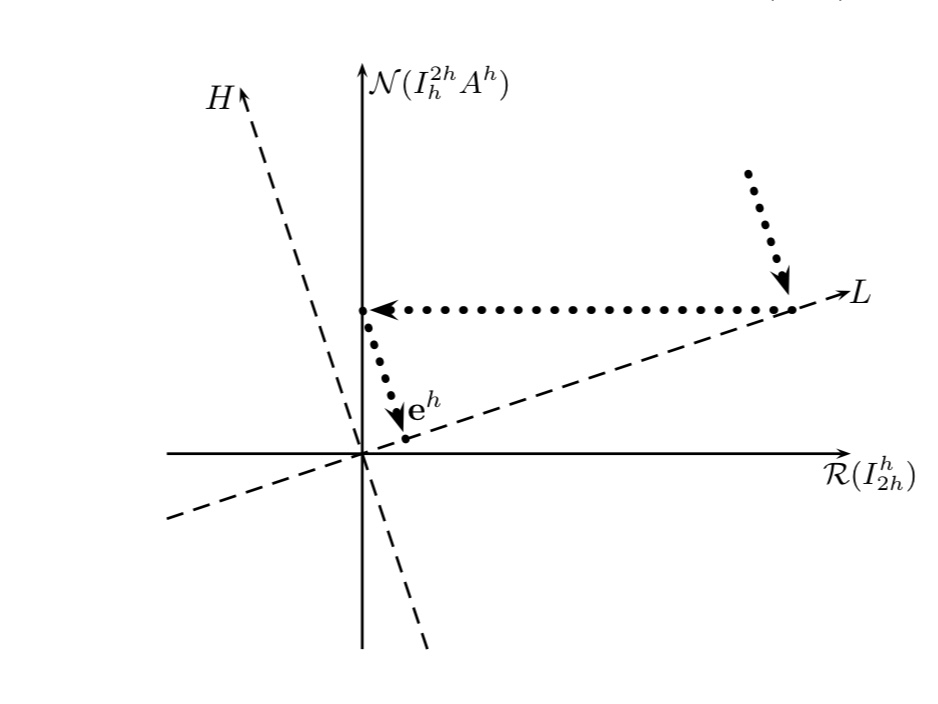
\includegraphics[scale=0.4]{../png/1.jpg}
\end{center}

\end{document}

%%% Local Variables: 
%%% mode: latex
%%% TeX-master: t
%%% End: 

